% vim: set spl=en:
\documentclass[smaller,t]{beamer}
\usepackage[utf8]{inputenc}
\usetheme{westlife}

\def\code#1{\structure{\texttt{#1}}}
\def\nadpis#1{\par\medskip\textbf{#1}}

\def\todo{{\color{red}\textbf{TODO}}}

\begin{document}
\makeatletter

\title{Virtualized Web Portals in EGI \\[\smallskipamount] Federated Cloud}
\date{MUSTweek, Brno, March 5--10}
\author[A. Křenek et al.]{Aleš Křenek, Radim Peša, Tomáš Raček, Vlastimil Holer, Daniel Kouřil, Ĺubomír Ontkoc}
\begin{frame}
\maketitle
\end{frame}

\begin{frame}{Why to virtualize web portals}
\begin{itemize}

\item{Web portal advantages}
\begin{itemize}
\item the user is scientist, not IT enthusiast
\item shield him/her from complexity of application and infrastructure
\item easy use, reproducible results
\end{itemize}

\item{Drawbacks}
\begin{itemize}
\item application and infra are complex, the portal is twice more
\item hand-crafted, ``don't touch and run for ever''
\end{itemize}

\item{Go to cloud}
\begin{itemize}
\item reproducible, automated deployment
\item for user: more flexible and scalable setup
\item for portal manager: more initial work but it pays
\end{itemize}
\end{itemize}

\end{frame}

\begin{frame}{Available software solutions}
\begin{itemize}
\item Many cloud orchestration and configuration management tools exist
\begin{itemize}
\item brief overview in West-life D4.1
\item thorough survey in INDIGO-Datacloud deliverables
\end{itemize}
\item Pragmatic choice for initial West-life solutions
\begin{itemize}
\item \textbf{Cloudify} -- cloud orchestration (before 1st INDIGO release was available)
\item \textbf{Puppet} -- configuration management (long term experience with us) 
\end{itemize}
\end{itemize}
\end{frame}

\begin{frame}{Typical portal architecture}
\begin{itemize}
\item Web front-end
\item Spool storage -- one folder per job 
\begin{itemize}
\item may have complex internal structure, long or short lived
\end{itemize}
\item  Machinery to handle computation
\begin{itemize}
\item triggered by changes in spool directory
\item either ``local'' lightweight calculation or remote jobs 
\end{itemize}
\item interface to AAI (user AuthN/Z, accouting)
\item interface to batch system or grid
\end{itemize}
\end{frame}

\begin{frame}{Final picture}
\begin{center}
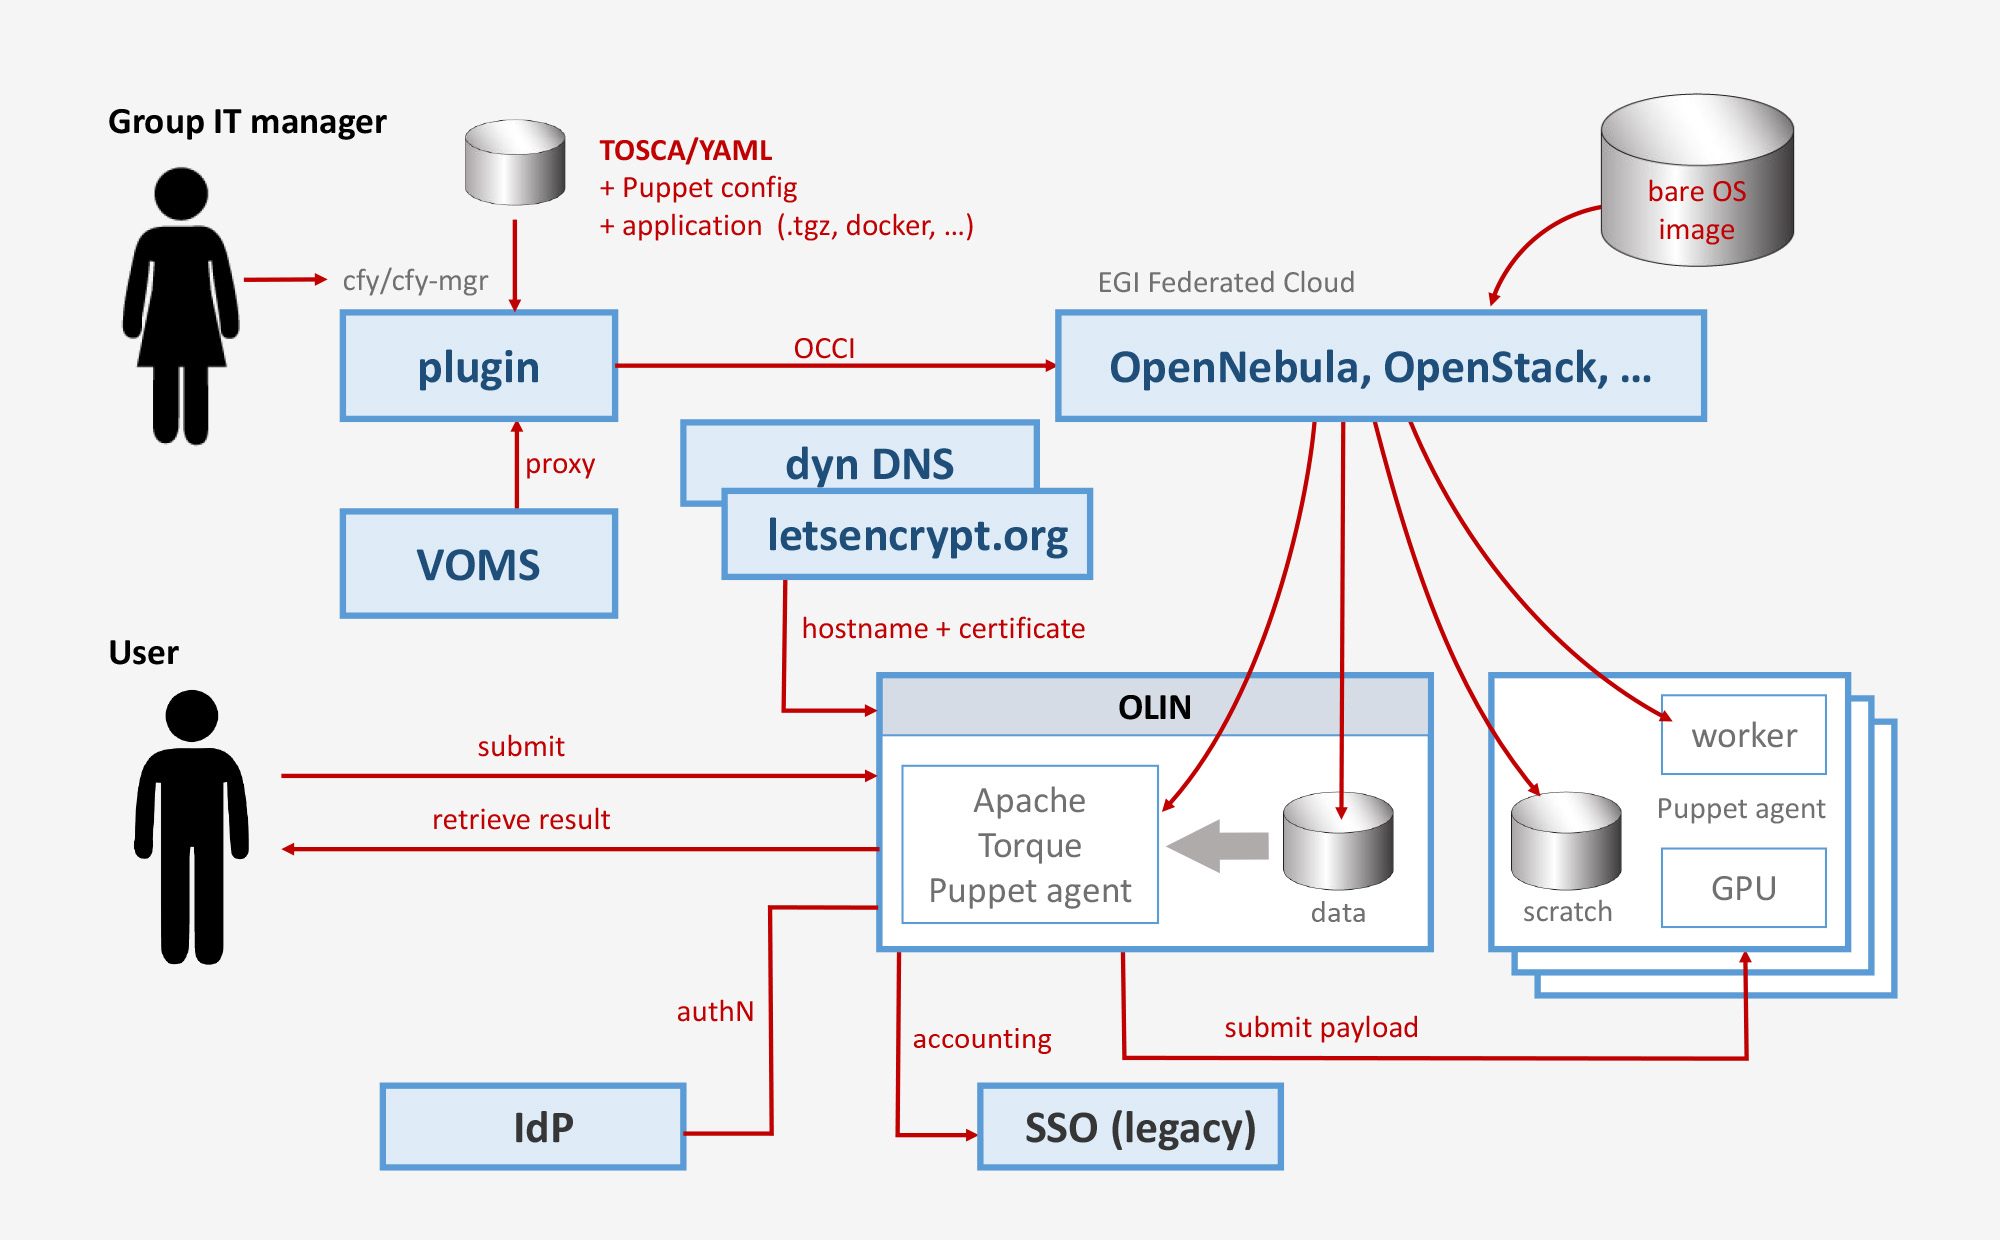
\includegraphics[width=.9\hsize]{P_virt.jpg}
\end{center}
\end{frame}

\begin{frame}{Deployment bottom-up}
\begin{itemize}
\item cloud nodes providers -- EGI FedCloud sites
\item cloud management systems -- OpenStack, OpenNebula, \dots (mostly hidden)
\item access interface -- OCCI, standard, hides management systems
\item orchestration (coordinated deployent) -- Cloudify (local, touches of CFM), Indigo solutions
\end{itemize}

\end{frame}

\begin{frame}{Deployment top-down}
\begin{itemize}
\item blueprint and node types
\begin{itemize}
\item node can be VM, installed software, specific configuration action, \dots
\item relationships among them (inclusion, dependencies, \dots)
\item lifecycle phases (create, configure, start, stop, \dots)
\end{itemize}
\item  inputs -- specific parameters for one deployment
\begin{itemize}
\item to keep the same blueprint
\end{itemize}
\item scripts to implement non-default lifecycle phases
\item resources -- any data used in at any stage
\begin{itemize}
\item ssh keys, configuration files, tarballs to expand, \dots
\end{itemize}
\item plugins
\begin{itemize}
\item highly modular architecture, anything can be (re)implemented by plugin
\item \textbf{fabric} -- execute remote commands
\item \textbf{occi} -- create VMs
\end{itemize}
\item software install and configuration
\begin{itemize}
\item Puppet -- the real way, used as blackbox today
\item hand-made scripts -- manageable in tutorial
\end{itemize}
\end{itemize}

\end{frame}

\begin{frame}{Tutorial overview}
\begin{itemize}
\item Understand the homework 
\begin{itemize}
\item obtain X.509 certificate and register it with VO
\item setup client environment -- software, CA certificates, VO servers, \dots (docker container)
\item check that occi works (interact with FedCloud site)
\item do the magic deployment out of blackbox 
\item \alert{let's understand it}
\end{itemize}
\item Deploy web application 
\begin{itemize}
\item start with non-claudified (but cleaned up) application code
\item \alert{extend Tosca description}
\item \alert{provide specific configuration scripts}
\end{itemize}
\end{itemize}
\end{frame}

\begin{frame}{Tutorial overview}
\begin{itemize}
\item Add worker node
\begin{itemize}
\item start with working web front end
\item pick another example -- Torque server + worker node
\item \alert{merge two Tosca specifications}
\item \alert{configure multi-node interaction}
\end{itemize}
\item Real-world user authentication
\begin{itemize}
\item start with working application with fake user
\item \alert{set up service provider and connect with IdP proxy}
\end{itemize}
\end{itemize}
\end{frame}


\begin{frame}{The application -- SAXS ensemble fit}
\begin{center}
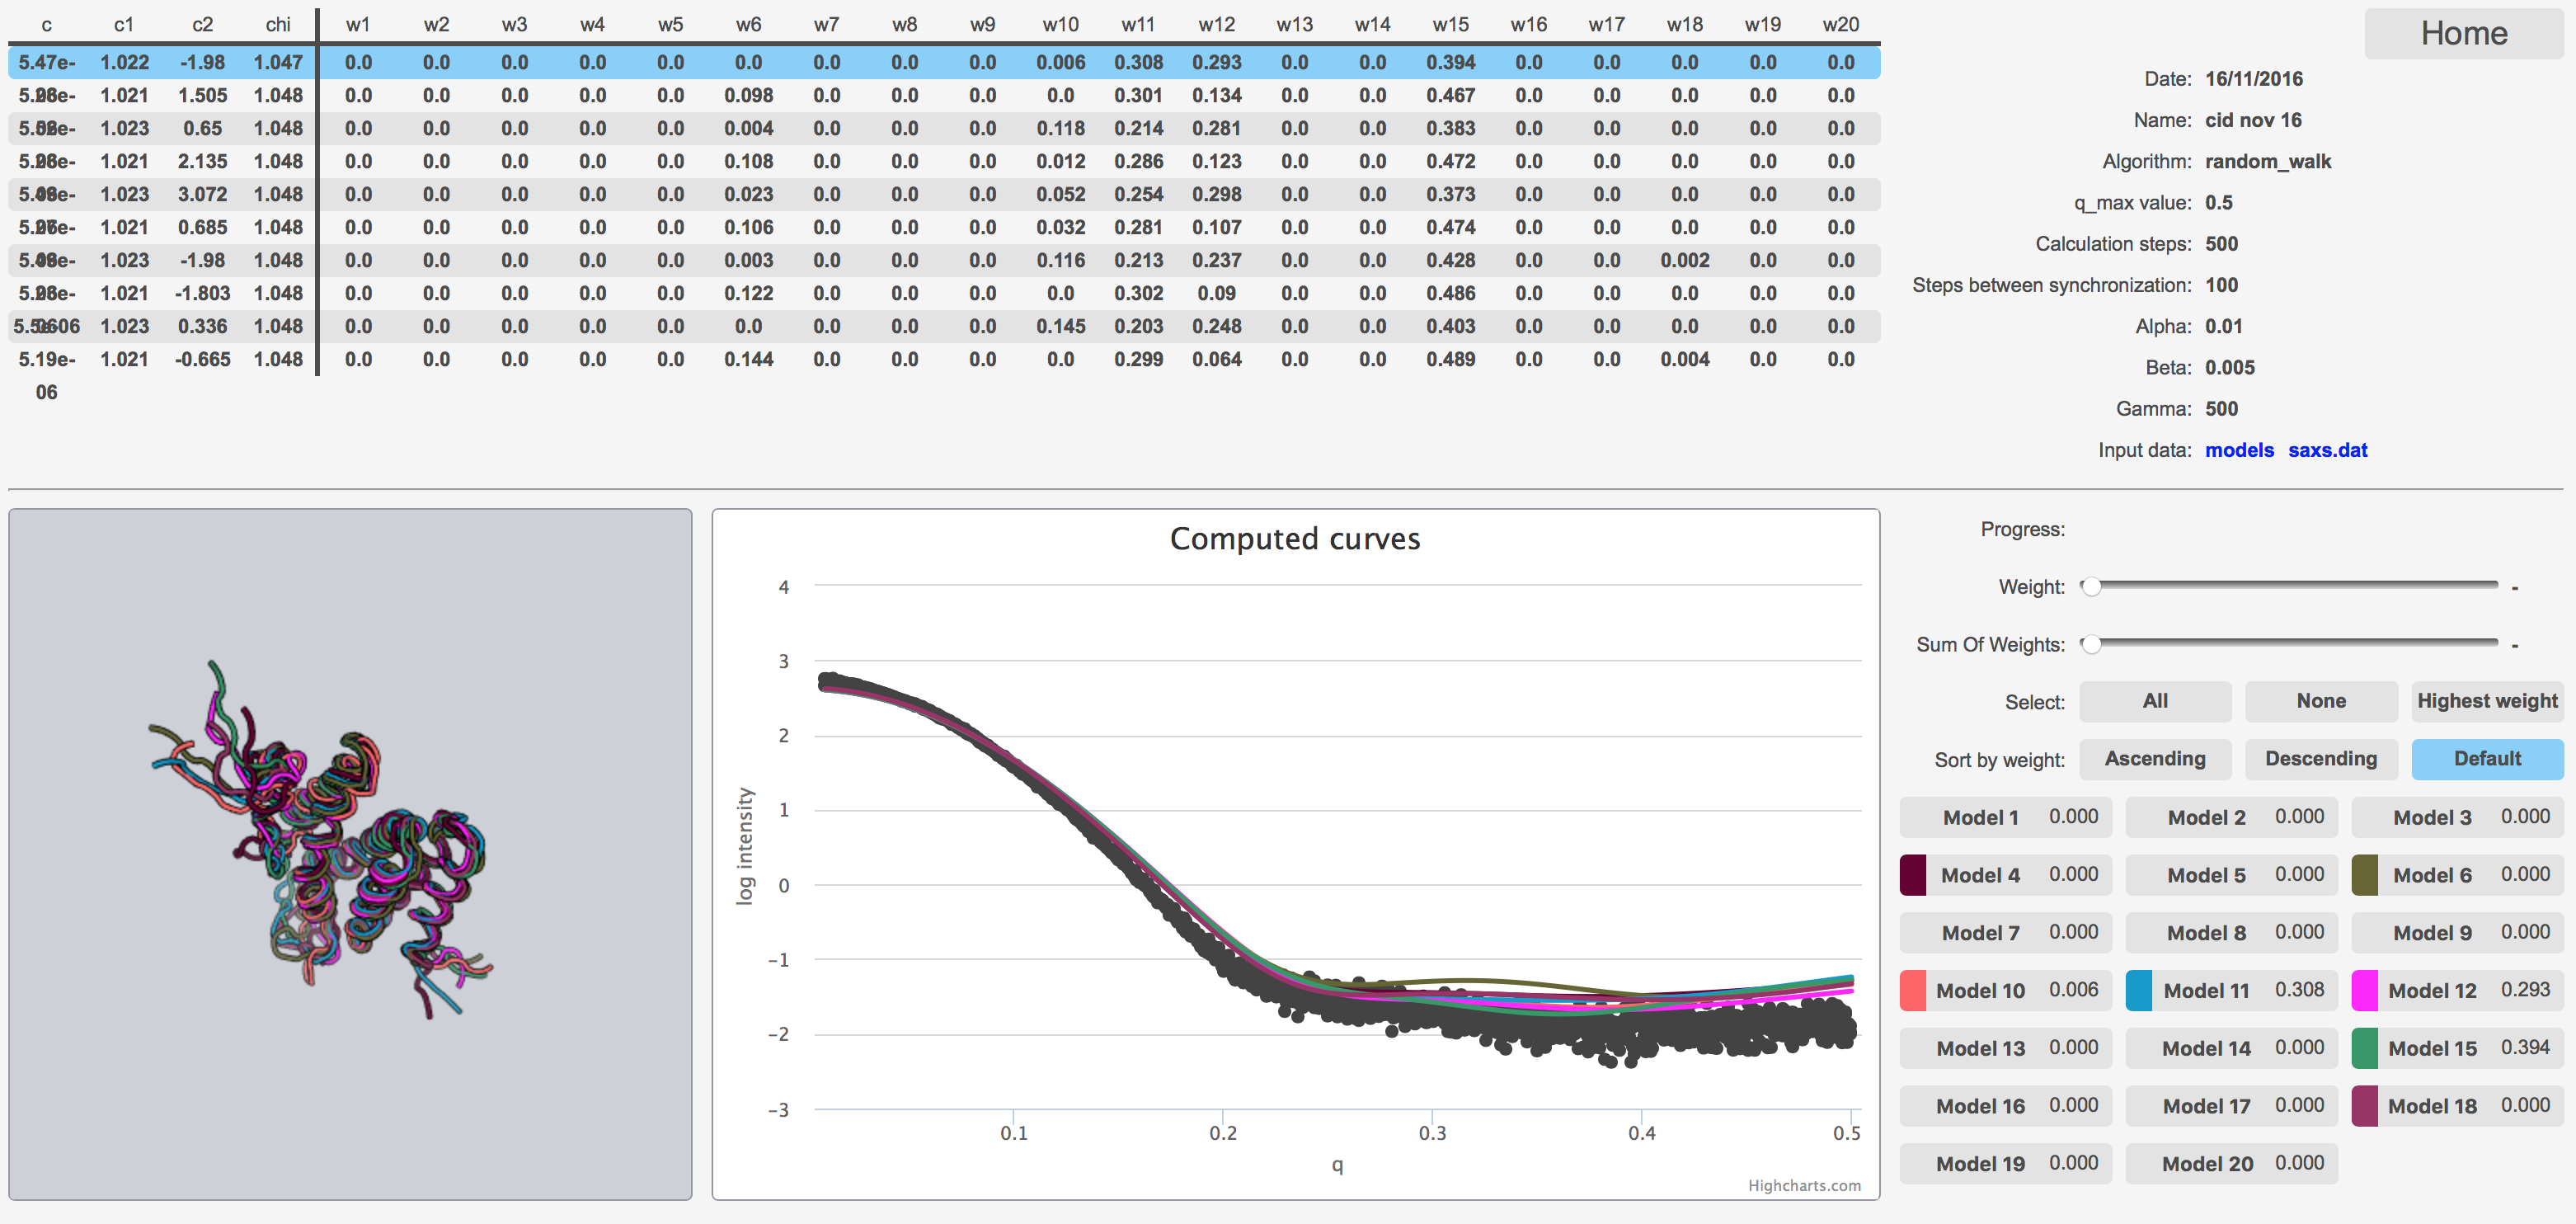
\includegraphics[width=.95\hsize]{saxs_cid}
\end{center}
\end{frame}

\begin{frame}{Bricks to be used}
\begin{itemize}
\item Apache server
\begin{itemize}
\item single node deployment
\item set up a VM using bare OS image (CentOS 7) using OCCI
\item use Puppet to configure Apache web server with ``Hello, world!'' CGI script
\item we will use it ``as is'', not touching internals (deployment scripts, Puppet recipes, \dots)
\end{itemize}

\item Torque server + worker node
\begin{itemize}
\item two node deployment
\item standalone, independent on the Apache one
\item complex Puppet configuration again
\end{itemize}
\end{itemize}
\end{frame}

\begin{frame}{Don't panic!}
\begin{itemize}
\item It is rather complex work, we know
\item Many things can go wrong
\item We will do the work step by step
\item Use local git commits to preserve work
\item Emergency checkpoints
\begin{itemize}
\item working implementations of the major steps
\item you can pick them if you get really lost 
\end{itemize}
\end{itemize}
\end{frame}



\begin{frame}{Understand the homework}
\begin{itemize}
\item In your Docker container (\code{radimpesa/mustweek2017})
\begin{itemize}
\item do a fresh clone of \code{git@github.com:ICS-MU/westlife-mustweek2017.git}
\item look into \code{apache/} folder
\end{itemize}

\item These slides in \code{talks/} folder
\item M4 preprocessing to distinguish local vs.\ CFM deployment 
\begin{itemize}
\item ignore today, just don't edit the generated \code{.yaml} files
\end{itemize}
\item browse the \code{.yaml} files and ask about their meaning
\begin{itemize}
\item blueprint and inputs in the main 
\item \code{types/} folder
\end{itemize}
\item briefly look into the deployment script 
\begin{itemize}
\item \code{scripts/puppet/runner.sh}
\item prepares and invokes Puppet 
\item this is the real stuff, no need to understand details now
\end{itemize}
\end{itemize}
\end{frame}

\begin{frame}{Understand the homework}
\begin{itemize}
\item Initialize Cloudify:\\ \code{\# source \$HOME/cfy/bin/activate}
\item Put something unique into:\\
\code{resources/puppet/site/helloworld/files/index.py}
\item Deploy:\\
\code{\# make clean \&\& make cfy-deploy}
\begin{itemize}
\item check the result, see:\\ \code{\# cfy local outputs}
\item ssh to the deployed node:\\
\code{\# ssh -i resources/ssh/id\_rsa cfy@\emph{the\_endpoint\_IP}}
\item point you web browser to:\\
\code{http://\emph{the\_endpoint\_IP}/cgi-bin/index.py}
\end{itemize}
\item Cleanup:\\
\code{\# make cfy-undeploy}
\end{itemize}
\end{frame}

\begin{frame}{Deploy web application}
\begin{itemize}
\item To speed up, start with the \code{apache/} example
\begin{itemize}
\item copy \code{Makefile}, blueprint and inputs, \code{types/}, and
\code{\{scripts,resources\}/puppet}
\end{itemize}
\item add ``software'' node to the blueprint
\begin{itemize}
\item contained in \code{apacheNode} (see \code{relationships} section)
\item started after \code{apache} node (\code{depens\_on} relationship)
\item use fabric plugin to start scripts
\end{itemize}
\item Installation, configuration, and start scripts
\begin{itemize}
\item ``poor-man'' quick solution (professional would use puppet \dots)
\item put them to \code{scripts/saxs-portal/}
\item runs unpriviledged -- use \code{sudo}
\item adapt (and break up) simple installation script and tarballs from \code{saxs/}
\item use \code{ctx} ``shell API'' to suck in cloudify resources (tarballs etc.) \\
\code{ctx download-resource resources/\emph{your/path/to/file} @\{"target\_path": "/tmp/destfile"\}'}
\end{itemize}
\end{itemize}
\end{frame}

\begin{frame}{Add worker node}
\begin{itemize}
\item Pick the other example in \code{torque/}
\begin{itemize}
\item appropriate pieces of blueprint and inputs
\item puppet resources (\code{manifests/} and \code{site/*}) -- just copy, no need to touch them
\item merge into results of previous step
\end{itemize}
\item Deploy application sofware to the worker node
\begin{itemize}
\item get inspiration from the web application deployment
\end{itemize}
\item generate SSH keys for the \code{saxs} user
\begin{itemize}
\item add key generation to Makefile
\item access it via \code{ctx} API in the installation script
\end{itemize}
\item Enable job management (\code{/usr/local/saxs/saxsd.sh})
\item \alert{It should work end-to-end now}
\begin{itemize}
\item test with sample data from \code{saxs/}
\end{itemize}
\end{itemize}

\end{frame}

\end{document}
